\documentclass[handout]{beamer}

\usetheme[progressbar=frametitle]{metropolis}
\metroset{block=fill}

\subtitle{NTIN071 Automata and Grammars}
\author{Jakub Bulín (KTIML MFF UK)}

\date{Spring 2025\\ 
    \vspace{1in} 
    \begin{flushleft}
        \it \footnotesize * Adapted from the Czech-lecture slides by Marta Vomlelová with gratitude. The translation, some modifications, and all errors are mine.
    \end{flushleft}
}

%% packages

\usepackage{amsmath}
\usepackage{amssymb}
\usepackage{amsthm}
\usepackage{cancel}
\usepackage{color}
\usepackage{colortbl}
\usepackage{forest}
\usepackage[utf8x]{inputenc}
\usepackage{multicol}
\usepackage{multirow}

%% colors
\definecolor{Gray}{gray}{0.9}

%% TikZ
\usepackage{tikz}
    \usetikzlibrary{
        automata,
        arrows,
        backgrounds,
        decorations.pathmorphing,
        fit,
        positioning,
        shapes,
        shapes.geometric,
        tikzmark
    } 
    \tikzset{>=stealth',shorten >=1pt,auto,node distance=2cm}
    \tikzset{initial text={}}
    \tikzset{elliptic state/.style={draw,ellipse}}

%% amsthm
\theoremstyle{plain}
    \newtheorem*{algorithm}{Algorithm}    
    \newtheorem*{observation}{Observation}
    \newtheorem*{proposition}{Proposition}

\theoremstyle{remark}
    \newtheorem*{exercise}{Exercise}
    \newtheorem*{remark}{Remark}

%% macros
\DeclareMathOperator{\RegE}{RegE}
\DeclareMathOperator{\RL}{RL}

% Just for Lecture 2
\newcommand{\x}{$\times$}
\newcommand{\nx}{\ }



\title{Lecture 12 -- Undecidable problems, Post's correspondence problem}


\begin{document}


\frame{\titlepage}


\begin{frame}{Recap of Lecture 11}
	
    \begin{itemize}        
        \item Recursively enumerable languages are exactly those generated by (Type 0) grammars
        \begin{itemize}
            \item TM to G: simulate moves on a reversed non-terminal copy of $\omega$, generate sufficient space, cleanup if accepting state
            \item G to TM: generate all strings, check if any of them represents a valid derivation of $\omega$ (sentential forms separated by $\#$)
        \end{itemize}   
        \item Context-sensitive languages:
        \begin{itemize}
            \item context-sensitive grammars are equivalent to monotone grammars
            \item Linear Bounded Automaton (LBA): nondeterministic TM with tape limited to the length of input
            \item constructions: monotone grammar to LBA, LBA to monotone grammar
        \end{itemize}
        \item Intro to computability: an overview
        \item decision problem $\leftrightsquigarrow$ the language of all `YES' instances
        \item machine-readable encoding of TMs
    \end{itemize}
	
\end{frame}



\begin{frame}{The Diagonal language}
    
    Let \alert{$\mathrm{decode}(w)$} be the TM $M$ such that $\mathrm{code}(M)=w$. (Recall: if $w$ is not a valid code, then $\mathrm{decode}(w)$ is a fixed one-state TM with no instructions.) Then:
    $$
    \alert{L_D}=\{w\mid w\notin L(\mathrm{decode}(w))\}
    $$
        
    \begin{theorem}
        $L_D$ is not recursively enumerable.
    \end{theorem}
    
    \textbf{Proof idea:} there cannot exist a TM recognizing $L_D$: running it on its own code would lead to Barber's paradox

    \bigskip

    \begin{quote}
        ``The program accepts all programs that don't accept themselves. Does the program accept itself?''
    \end{quote}

\end{frame}


\begin{frame}{Proof that $L_D=\{w\mid w\notin L(\mathrm{decode}(w))\}$ is not RE}

    \textbf{Proof:} Assume for contradiction that $L_D=L(M)$ for some $M$. Let $w=\mathrm{code}(M)$. Then $L_D=\{w\mid w\notin L(M)\}$. Is $w\in L(M)$?
    $$
    w\in L(M)\ \Leftrightarrow\ w\in L_D\ \Leftrightarrow\ w\notin L(M)
    $$
    
    \vspace{-24pt}
    \hfill\qedsymbol

    Why `diagonal'? A variant of Cantor's diagonal argument. Order all TMs by  $M_i=\mathrm{decode}(w_i)$. Does $M_i$ accept $w_j$?

    \vspace{-12pt}
    \begin{center}
        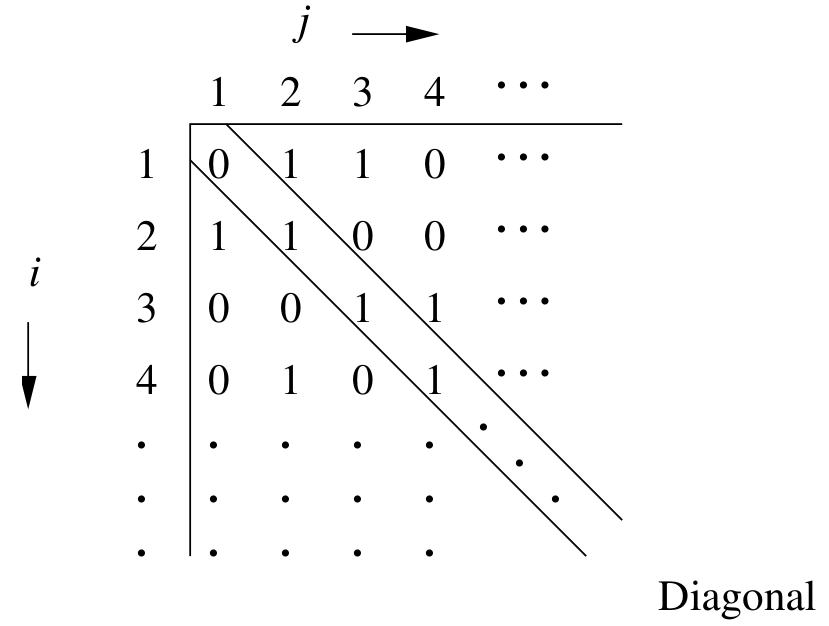
\includegraphics[width=0.48\textwidth]{files/diagonal.PNG}
    \end{center}
    \vspace{-15pt}
    A TM for $L_D$ would be one of the rows but differs from each row in the diagonal element. (Same as the proof that $\mathbb R$ is uncountable.)  
    
\end{frame}


\begin{frame}{The Universal Turing Machine}

    The \alert{Universal Turing Machine} $U$ can simulate any TM (given by its code) on any input. More precisely, $U$ accepts exactly inputs of the form \alert{$\langle \mathrm{code}(M),w\rangle$} where \alert{$w\in L(M)$}.
       
    \begin{columns}

        \column{0.5\textwidth}
        
        \textbf{The construction:}  four tapes
        \begin{enumerate}
            \item input tape ($w$ and the encoded transitions of $M$)
            \item simulated tape of $M$, symbols encoded as $0^i$, separated by 1s
            \item state of $M$, again represented by $0^i$
            \item scratch tape
        \end{enumerate}
    
        \column{0.5\textwidth}

        \begin{center}
            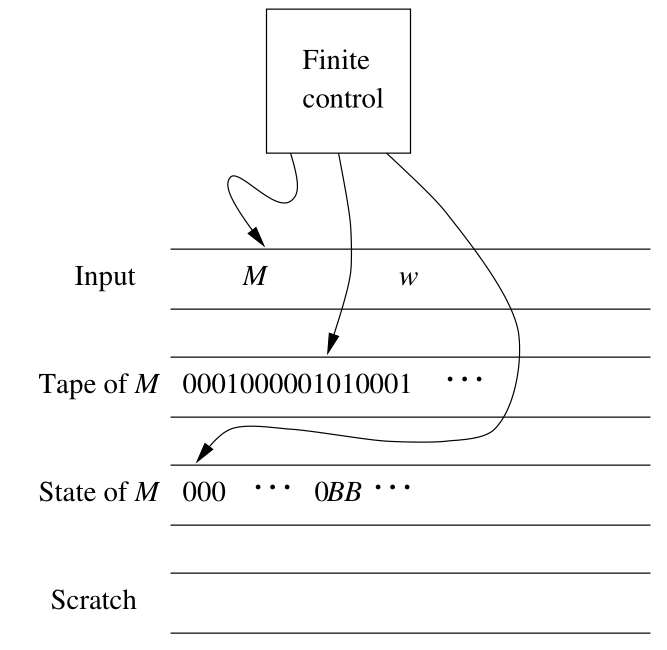
\includegraphics[width=\textwidth]{files/universalTM.PNG}
        \end{center}        
        
    \end{columns}

\end{frame}


\begin{frame}{The operation of $U$}

    \small
    \vspace{-3pt}
    \textbf{Initialize:}
    \vspace{-9pt}
    \begin{itemize}
        \item Check if the input code is valid, if not, halt without accepting
        \item Initialize Tape 2 with $w$ in its encoded form: $10$ for $0$ in $w$, $100$ for $1$\\ 
        Blanks are left blank and replaced with $1000$ only `on demand'\\ 
        Move 2nd head to the first simulated cell. 
        \item Place $0$ (the start state of $M$) on Tape 3.
    \end{itemize}
    \vspace{-3pt}
    \textbf{Simulate moves of $M$:}
    \vspace{-9pt}
    \begin{itemize}
            \item Search Tape 1 for the appropriate transition $0^i10^j10^k10^\ell10^m$, where $0^i$ on Tape 3, $0^j$ on Tape 2.
            \item Change the content of Tape 3 to $0^k$.
            \item Replace $0^j$ on Tape 2 by $0^\ell$. Scratch tape to manage spacing.
            \item Move head on Tape 2 to the next $1$ left or right, depending on $m$.
    \end{itemize}
    \vspace{-3pt}
    \textbf{Termination:} If $M$ has no transition matching simulated state \& tape symbol, halt without accepting. If $M$ enters accepting state, $U$ accepts.

\end{frame}


\begin{frame}{Recursive languages are closed under complement}

    \begin{lemma}
        If $L$ is recursive, then $\overline{L}$ is recursive as well.
    \end{lemma}

    \begin{center}
        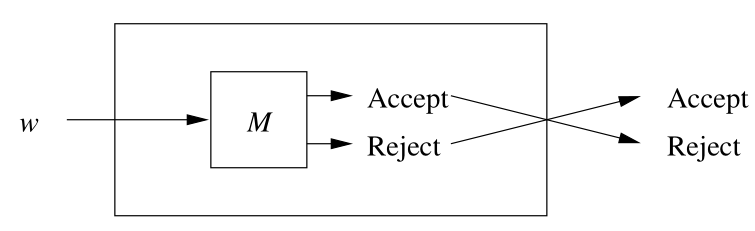
\includegraphics[width=0.7\textwidth]{files/compRec.PNG}
    \end{center}

    \textbf{Proof:} Given $M$ deciding $L$, construct $M'$ deciding $L'$. Since $M$ always halts, if it does not accept, the reason is missing transition. 
    
    \medskip $M'$ has a single, new accepting state $q_\text{ACCEPT}$. For every non-accepting state of $M$ and every tape symbol $X$ such that $\delta(q,X)$ is undefined, redefine $\delta'(q,X)=(q_\text{ACCEPT},X,L)$. 
    

    Clearly, $L(M')=\overline{L}$. Since $M$ is guaranteed to halt, so is $M'$.\hfill\qedsymbol    

\end{frame}


\begin{frame}{Post's theorem}

    \begin{theorem}
        $L$ is recursive iff both $L$ and $\overline{L}$ are recursively enumerable.
    \end{theorem}
    \vspace{-6pt}
    \textbf{Proof:} \alert{$\Rightarrow$} Follows from the lemma.
    \\ \alert{$\Leftarrow$} Let $L=L(M_1)$ and $\overline{L}=L(M_2)$. For an input $w$, simulate both $M_1$ and $M_2$ (two tapes, states with two components). $L$ and $\overline{L}$ are complementary, one of $M_1$ or $M_2$ will halt and accept.

    \vspace{-3pt}
    \begin{itemize}
        \item If $M_1$ accepts, accept.
        \item If $M_2$ accepts, reject.\hfill\qedsymbol
    \end{itemize}

    \vspace{-6pt}
    \begin{center}
        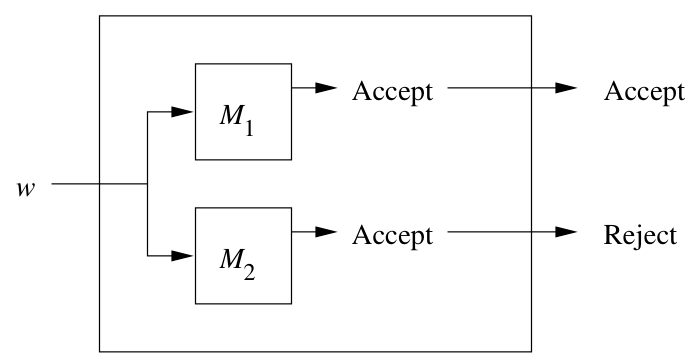
\includegraphics[width=0.6\textwidth]{files/bothRE.PNG}
    \end{center}

\end{frame}


\begin{frame}{The Universal language and its undecidability}

    $L_U=\{\langle \mathrm{code}(M),w\rangle\mid w\in L(M)\}$\hfill RE but not R\\
    $\overline{L_D}=\{w\mid w\in L(\mathrm{decode}(w))\}$\hfill RE but not R\\
    $L_D=\{w\mid w\notin L(\mathrm{decode}(w))\}$\hfill not RE

    \medskip

    \begin{theorem}
        The Universal language is recursively enumerable but not recursive. Same is true for complement of the Diagonal language.
    \end{theorem}    

    \vspace{-6pt}
    \textbf{Proof:}
    \vspace{-6pt}
        \begin{itemize}
            \item \alert{$L_U$ is RE:} it is recognized by the Universal TM $U$
            \item \alert{$\overline{L_D}$ is RE:} rewrite input $w$ to $\langle w,w\rangle=w111w$, then run on $U$
            \item \alert{$\overline{L_D}$ is not recursive:} if it were, by Post's theorem $L_D$ would be RE (actually R), but we know it is not
            \item \alert{$L_U$ is not recursive:} if it were, $\overline{L_D}$ would be recursive (rewrite $w$ to $\langle w,w\rangle$, run on the hypothetical $M$ deciding $L_U$)\hfill\qedsymbol
        \end{itemize}

\end{frame}


\begin{frame}{Reductions between decision problems}

    \begin{definition}
        A \alert{reduction} $R$ is an algorithm mapping all instances of $P_1$ to instances of $P_2$ that always halts, and for every instance $w$ of $P_1$ outputs an instance $R(w)$ of $P_2$ such that:
        \begin{itemize}
            \item $w$ is a YES instance of $P_1$ iff $R(W)$ is a YES instance of $P_2$
            \item $w$ is a NO instance of $P_1$ iff $R(W)$ is a NO instance of $P_2$
        \end{itemize}
        (Technically, $R=f_M$ for some TM $M$ that always halts.)
    \end{definition}
    
    \textbf{Example} The mapping $w\rightsquigarrow \langle w,w\rangle=w111w$ (from the previous proof) can clearly be done algorithmically. It is a reduction from $\overline{L_D}$ to $L_U$ (and also from $L_D$ to $\overline{L_U}$).

\end{frame}


\begin{frame}{Only easy reduce to easy, hard only reduce to hard}

    \begin{theorem}
        If there is a reduction from $P_1$ to $P_2$, then:
        \begin{enumerate}[(i)]            
            \item If $P_1$ is not decidable then neither is $P_2$.
            \item If $P_2$ is decidable, then so is $P_1$.
            \item If $P_1$ is not partially decidable then neither is $P_2$. 
            \item If $P_2$ is partially decidable, then so is $P_1$.
        \end{enumerate}
    \end{theorem}

    %\textbf{Proof:}
    \begin{itemize}
        \item[(i\&ii)] Let $P_1$ be undecidable. If $P_2$ were decidable, we could combine the reduction from $P_1$ to $P_2$ with the algorithm deciding $P_2$ to construct an algorithm that decides $P_1$.
        \item[(iii\&iv)] Assume $P_1$ is not partially decidable, but $P_2$ is. Similarly as above, we could combine the reduction and the algorithm for $P_2$ to get an algorithm partially deciding $P_1$--a contradiction.\hfill\qedsymbol
    \end{itemize}       

\end{frame}



\begin{frame}{``Does the given program halt for the given input?'}

    An instance of the \alert{Halting Problem} $\mathrm{Halt}$: $\langle \mathrm{code}(M),w\rangle\in \{0,1\}^*$. The answer is YES iff $M$ halts on input $w$; otherwise it is NO. 

    
    \begin{theorem}
        The Halting Problem is undecidable.
    \end{theorem}
    (Note that it is partially decidable: we can simulate using $U$.)

    \textbf{Proof:} Reduce the undecidable problem $\overline{L_D}$ to $\mathrm{Halt}$. Given an instance $w$ of $\overline{L_D}$, let $M=\mathrm{decode}(w)$. Modify $M$ to get $M'$ such that if $M$ \alert{halts without accepting}, $M'$ \alert{goes to an infinite loop}.

    Set \alert{$R(w)=\langle \mathrm{code}(M'),w\rangle$}. Clearly, it can be done algorithmically.

    \begin{itemize}
        \item If $w\in\overline{L_D}$, i.e. $w\in L(M)$, then $M'$ accepts (thus halts) on $w$.
        \item If $w\notin\overline{L_D}$, i.e. $w\notin L(M)$, then either $M$ doesn't halt or halts without accepting. In either case $M'$ doesn't halt on $w$. \hfill\qedsymbol
    \end{itemize}


\end{frame}


\begin{frame}{Accepts no inputs?}

    %Define the languages $L_e, L_{ne}\in \{0,1\}^*$ as follows:
    \begin{itemize}
        \item $L_e=\{\mathrm{code(M)}\mid L(M)=\emptyset\}$
        \item $L_{ne}=\{\mathrm{code(M)}\mid L(M)\neq\emptyset\}=\overline{L_e}$
    \end{itemize}

    \begin{theorem}
        \begin{enumerate}[(i)]
            \item $L_{e}$ is not recursively enumerable.
            \item $L_{ne}$ is recursively enumerable but not recursive.
        \end{enumerate}
    \end{theorem}

    \textbf{Proof:} As $L_{ne}=\overline{L_{e}}$, \alert{(i) follows from (ii)} by Post's theorem.

    \medskip

    \alert{$L_{ne}$ is RE:} nondeterministically guess $w\in L(M)$, verify using $U$
 
    \begin{center}
        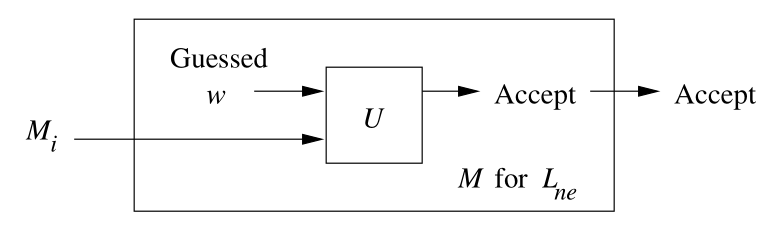
\includegraphics[width=0.8\textwidth]{files/Lne.PNG}
    \end{center}

\end{frame}


\begin{frame}{Proof cont'd}

    \alert{$L_{ne}$ is not recursive:} reduction from undecidable $\overline{L_D}$

    Given $w=\mathrm{code(M)}$, $R(w)$ is a TM $M'$ that ignores its input, rewrites the input tape with $w$, and simulates $M$ on $w$. 

    \begin{center}
        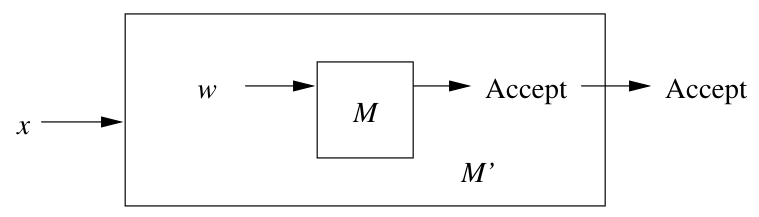
\includegraphics[width=0.8\textwidth]{files/Lne2.PNG}
    \end{center}
    
    \begin{itemize}
        \item If $w\in\overline{L_D}$, i.e. $w\in L(M)$, then $R(w)$ always accepts.
        \item If $w\notin\overline{L_D}$, i.e. $w\notin L(M)$, then $R(w)$ never accepts.\hfill\qedsymbol
    \end{itemize}

\end{frame}


\begin{frame}{Rice's theorem}

    Which properties of programs are decidable?

    \bigskip

    None of them!

    \bigskip

    (Except for trivial properties true/false for all programs.)

    \bigskip

    We have all the tools, but not the time to prove \href{https://en.wikipedia.org/wiki/Rice\%27s\_theorem}{\alert{Rice's theorem}}.

    \bigskip

    ``Theoretically, static analysis of programs cannot be done automatically?''

\end{frame}


\begin{frame}{Summary of Lecture 12}

    \begin{itemize}
        \item the Diagonal language $L_D$ is not recursively enumerable
        \item the Universal language $L_U$, the Universal TM: simulate any $M$ on any $w$
        \item recursive languages are closed under complement
        \item Post's theorem: $L$ recursive iff both $L,\overline{L}$ are RE
        \item $L_U$, $\overline{L_D}$ are recursively enumerable but not recursive
        \item reductions between decision problems
        \item the Halting problem is undecidable        
        \item (Rice's thm: nontriv. properties of programs are undecidable)
    \end{itemize}

\end{frame}


\end{document}
